\documentclass[11pt,a4paper]{article}

\usepackage[margin=2.5cm]{geometry}
\usepackage{graphicx}
\usepackage{amsmath, amssymb}
\usepackage{booktabs}
\usepackage{hyperref}
\usepackage{setspace}

\usepackage[labelfont=bf]{caption}
\usepackage{subcaption}
\captionsetup[subfigure]{justification=centering,singlelinecheck=false}

\usepackage{pgfplots}
\pgfplotsset{compat=newest}

\usepackage{multirow}

\newcommand{\unitname}{Understanding Deep Learning}
\newcommand{\assignmenttitle}{Age and Gender Prediction with CNNs}
\newcommand{\authorname}{Rithvik Marreddy}

% Model links (edit these with your actual shared URLs)
\usepackage[hidelinks]{hyperref}

\newcommand{\modelAlink}{%
  \href{https://drive.google.com/file/d/1IopVGb6fbhNIXqgFGUXBufDDIlO_xU22/view?usp=drive_link}{\texttt{age\_gender\_A.keras}}%
}
\newcommand{\modelBlink}{%
  \href{https://drive.google.com/file/d/1ok4jF9eWFTqmg7UVxBWfj6GsbcN_gapG/view?usp=drive_link}{\texttt{age\_gender\_B.keras}}%
}

\begin{document}

\begin{titlepage}
    \thispagestyle{empty}
    \begin{center}
        \vspace*{2cm}
        
        % Unit name (smaller heading)
        {\Large \textsc{\unitname} \par}
        
        \vspace{1.5cm}
        
        % MAIN COURSEWORK TITLE – big and bold
        {\Huge \bfseries Age and Gender Prediction with CNNs \par}
        
        
        \vspace{14cm}

        
        % Model links
        \begin{flushleft}
        \textbf{Model files (shared links):}
        \begin{itemize}
            \item \textbf{age\_gender\_A.keras (Custom CNN from scratch):}\\
            \modelAlink
            \item \textbf{age\_gender\_B.keras (Pre-trained CNN fine-tuned on this dataset):}\\
            \modelBlink
        \end{itemize}
        \end{flushleft}
        
    \end{center}
\end{titlepage}

\onehalfspacing


\section{Introduction} % 200 words
This coursework investigates the use of a convolutional neural network (CNN) to predict the ages and genders of people from facial images. The two models explored are a custom designed CNN and a pretrained model (from ImageNet) that is fine-tuned for the same task. The dataset consists of 5000 facial images with age and gender labels that is split in a 80:20 ratio across the training and validation datasets. \autoref{table1} and \autoref{figure1} show the age and gender distributions of the training and validation datasets, showing that the validation dataset is chosen to mirror the training data. 

\begin{table}[h!]
\centering
\renewcommand{\arraystretch}{1.15} % a bit more vertical space
\begin{tabular}{||l|r|r|r|r||}
 \hline
 Gender & Train count & Train (\%) & Val count & Val (\%) \\ [0.5ex]
 \hline\hline
 Female & 1937 & 48.4 &  479 & 47.9 \\
 Male   & 2063 & 51.6 &  521 & 52.1 \\ [0.5ex]
 \hline
 Total  & 4000 & 100.0 & 1000 & 100.0 \\ [0.5ex]
 \hline
\end{tabular}
\caption{Gender distribution in the training and validation sets.}
\label{table1}
\end{table}

\begin{figure}[ht]
  \centering

  \begin{subfigure}[b]{0.45\textwidth}
    \centering
    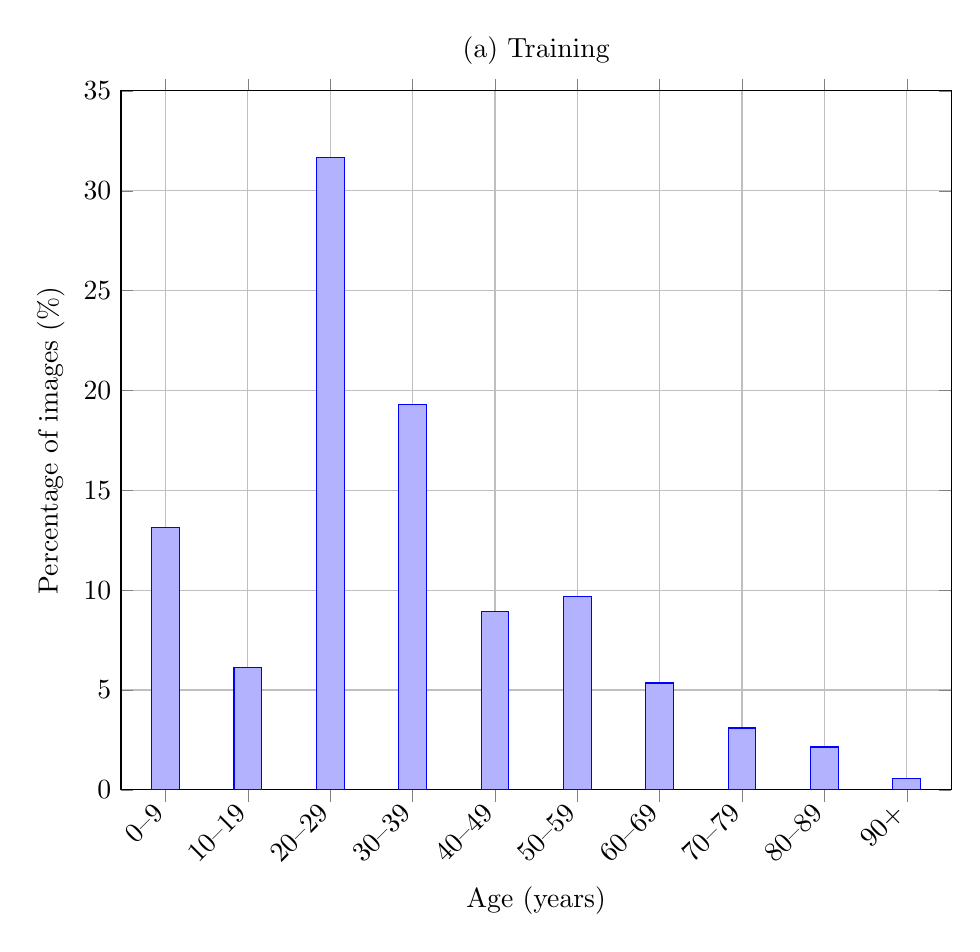
\begin{tikzpicture}
      \begin{axis}[
        width=\linewidth,
        ybar,
        bar width=10pt,
        xlabel={Age (years)},
        ylabel={Percentage of images (\%)},
        title={(a) Training},
        symbolic x coords={0--9,10--19,20--29,30--39,40--49,
                           50--59,60--69,70--79,80--89,90+},
        xtick=data,
        xticklabel style={rotate=45, anchor=east},
        ymin=0,
        ymax=35,
        grid=major,
        enlarge x limits=0.06,
      ]
        \addplot coordinates {
          (0--9,13.15)
          (10--19,6.15)
          (20--29,31.65)
          (30--39,19.28)
          (40--49,8.92)
          (50--59,9.70)
          (60--69,5.35)
          (70--79,3.10)
          (80--89,2.15)
          (90+,0.55)
        };
      \end{axis}
    \end{tikzpicture}
    \label{subfig:age_train}
  \end{subfigure}
  \hspace{0.05\textwidth}
  \begin{subfigure}[b]{0.45\textwidth}
    \centering
    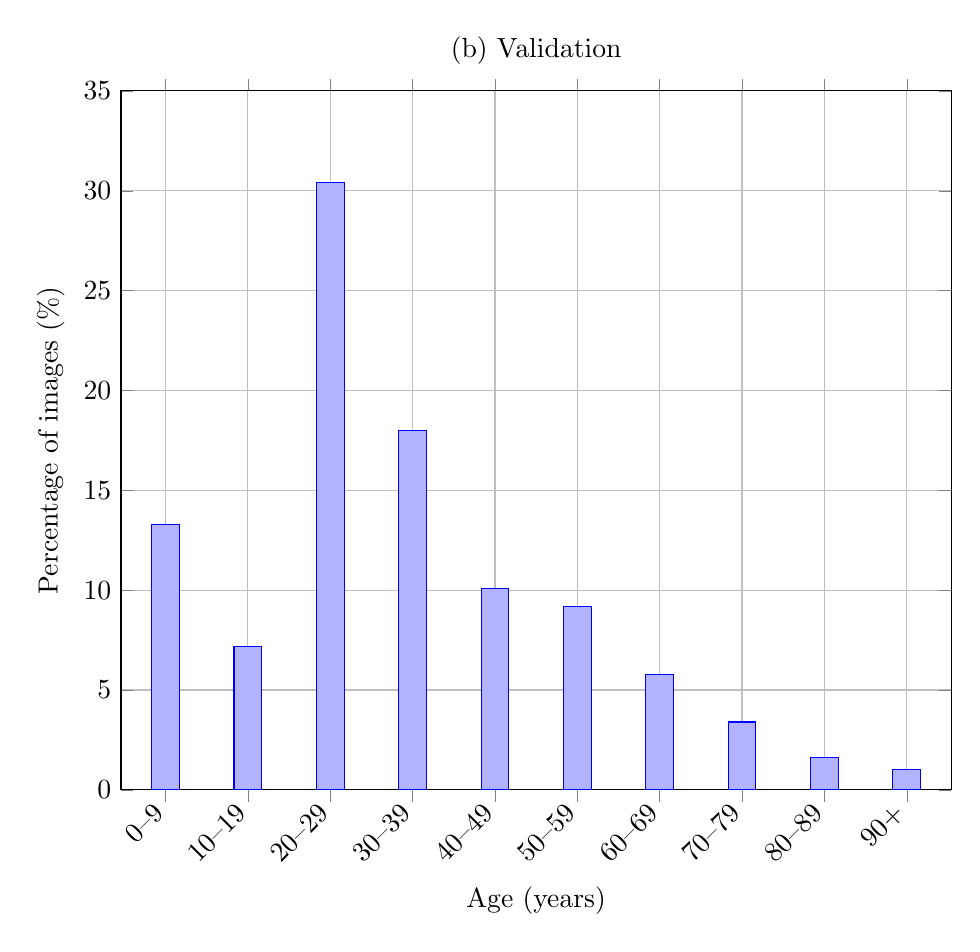
\begin{tikzpicture}
      \begin{axis}[
        width=\linewidth,
        ybar,
        bar width=10pt,
        xlabel={Age (years)},
        ylabel={Percentage of images (\%)},
        title={(b) Validation},
        symbolic x coords={0--9,10--19,20--29,30--39,40--49,
                           50--59,60--69,70--79,80--89,90+},
        xtick=data,
        xticklabel style={rotate=45, anchor=east},
        ymin=0,
        ymax=35,
        grid=major,
        enlarge x limits=0.06,
      ]
        \addplot coordinates {
          (0--9,13.3)
          (10--19,7.2)
          (20--29,30.4)
          (30--39,18.0)
          (40--49,10.1)
          (50--59,9.2)
          (60--69,5.8)
          (70--79,3.4)
          (80--89,1.6)
          (90+,1.0)
        };
      \end{axis}
    \end{tikzpicture}
    \label{subfig:age_val}
  \end{subfigure}

  \caption{Training and validation age distributions in 10-year bins. Ages ranging from 0 - 116 years.}
  \label{figure1}
\end{figure}

\begin{figure}[ht]
  \centering
  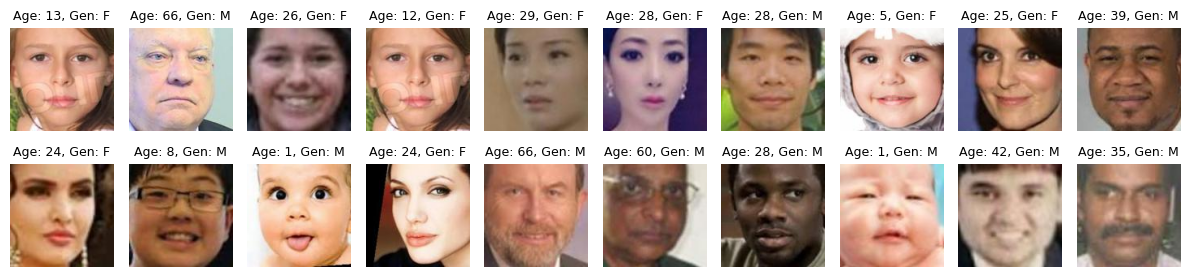
\includegraphics[width=\linewidth]{figure2.png} % or images/figure2.png
  \caption{Example training images with age and gender labels.}
  \label{figure2}
\end{figure}

\subsection{Data Augmentation}
The face images are resized to an input shape of (128x128x3) representing RGB colours, which are normalised to the [0,1] range, allowing gradient optimisers to work more consistently and reducing the issue of exploding or vanishing gradients \cite{pradhan2022normalization}. 

The CNN faces the challenge of overfitting due to a small dataset. Data augmentation is applied to only the training data to expand the dataset and add some variation. This is applied using Keras' pre-processing layers and is not applied to the validation set so that it remains a valid test to see the model's performance. 

\begin{figure}[ht]
  \centering
  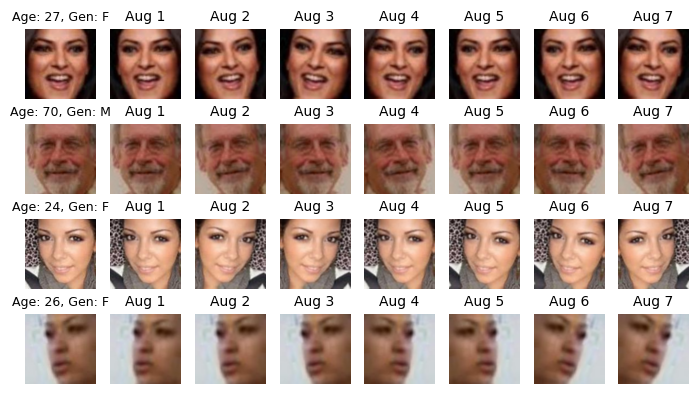
\includegraphics[width=\linewidth]{figure3.png}
  \caption{Example training images after data augmentation:
  \texttt{RandomFlip("horizontal")}, \texttt{RandomRotation(0.03)},
  \texttt{RandomZoom(0.01)}.}
  \label{figure3}
\end{figure}

Unlike facial recognition problems, age estimation requires the dataset to preserve details such as wrinkles, skin texture, and under-eye shadows \cite{zenodo2024agegender}. This means that minimal augmentation is used, avoiding methods to alter colour, blurring, or aggressive cropping. \autoref{figure3} displays the augmentation, where minimal augmentation is used to prevent the model from learning features that don't exist in the validation set. 

% include if word count allows to. 
% The choice to implement augmentation using the map() function within the data pipeline enables on-the-fly preprocessing, applying transformations dynamically during training without inflating dataset size or memory usage. This design ensures that data augmentation remains modular and external to the model architecture, allowing the CNN structure to remain unchanged while maintaining efficient and scalable training.

\section{The Custom CNN (Model A)} % 500

\subsection{Model Structure}

\begin{table}[h!]
\centering
\renewcommand{\arraystretch}{1.15}
\begin{tabular}{||l|c|c|c|c||}
 \hline
 Layer & Filters & Output & Kernel Size & Activation fn \\ [0.5ex]
 \hline\hline
 Input image        & -    & $128 \times 128 \times 3$   & -          & -      \\
 \hline
 Conv1a             & 32   & $128 \times 128 \times 32$  & $3 \times 3$ & ReLU  \\
 Conv1b             & 32   & $128 \times 128 \times 32$  & $3 \times 3$ & ReLU  \\
 MaxPooling1        & -    & $64 \times 64 \times 32$    & $2 \times 2$ & -     \\
 Dropout1           & -    & $64 \times 64 \times 32$    & -          & -      \\
 \hline
 Conv2a             & 64   & $64 \times 64 \times 64$    & $3 \times 3$ & ReLU  \\
 Conv2b             & 64   & $64 \times 64 \times 64$    & $3 \times 3$ & ReLU  \\
 MaxPooling2        & -    & $32 \times 32 \times 64$    & $2 \times 2$ & -     \\
 Dropout2           & -    & $32 \times 32 \times 64$    & -          & -      \\
 \hline
 Conv3a             & 128  & $32 \times 32 \times 128$   & $3 \times 3$ & ReLU  \\
 Conv3b             & 128  & $32 \times 32 \times 128$   & $3 \times 3$ & ReLU  \\
 MaxPooling3        & -    & $16 \times 16 \times 128$   & $2 \times 2$ & -     \\
 Dropout3           & -    & $16 \times 16 \times 128$   & -          & -      \\
 \hline
 Conv4a             & 256  & $16 \times 16 \times 256$   & $3 \times 3$ & ReLU  \\
 Conv4b             & 256  & $16 \times 16 \times 256$   & $3 \times 3$ & ReLU  \\
 MaxPooling4        & -    & $8 \times 8 \times 256$     & $2 \times 2$ & -     \\
 Dropout4           & -    & $8 \times 8 \times 256$     & -          & -      \\
 \hline
 GlobalAvgPooling   & -    & $256$                       & -          & -      \\
 Shared FC          & 512  & $512$                       & -          & ReLU  \\
 Shared Dropout     & -    & $512$                       & -          & -      \\
 \hline\hline
 \multicolumn{5}{||c||}{\textbf{Gender Branch}} \\
 \hline
 Gender FC          & 128  & $128$                       & -          & ReLU  \\
 Gender Dropout     & -    & $128$                       & -          & -      \\
 Gender output      & 1    & $1$                         & -          & Sigmoid \\
 \hline\hline
 \multicolumn{5}{||c||}{\textbf{Age Branch}} \\
 \hline
 Age FC1            & 256  & $256$                       & -          & ReLU  \\
 Age Dropout1       & -    & $256$                       & -          & -      \\
 Age FC2            & 128  & $128$                       & -          & ReLU  \\
 Age Dropout2       & -    & $128$                       & -          & -      \\
 Age output         & 1    & $1$                         & -          & Linear \\
 \hline
\end{tabular}
\caption{Architecture of Model A}
\label{table2}
\end{table}

Model A is a custom multi-output CNN designed to predict both age and gender from the normalised input facial images of shape (128x128x3). The network architecture consists of four convolutional blocks shown in \autoref{table2}. Stacking two 3x3 convolutions has a receptive field equivalent to a single 5x5 filter but uses fewer parameters than a single kernel. To ensure generalisation of the model, dropout layers are used with increasing rates, while Batch Normalisation occurs between convolution layers, that standardises the inputs after activation, thereby accelerating convergence.

To ensure the final feature map remains under 10 x 10, the model applies 2x2 max pooling layers at each step which halves the resolution of the output. This output is processed by a GlobalAveragePooling2D layer, which converts the 3D feature map into a 256-demnsional vector. This method is preferred over flatten as it acts as a regulariser, improving the model's robustness to geometric shifts \cite{lin2013network}. 

These pooled features are passed to a shared 512-unit Dense layer activated by ReLU and followed by a larger dropout. This forces the model to capture high-level details that are important for both age and gender branches while also reducing the risk of overfitting. After the shared fully connected layer, the model splits into the age and gender branches. Since age is a continuous output that is harder to map, the model uses two fully connected layers to provide the depth for model required to capture subtle features. The lower dropout helps retain important features for the regression task. 

The model combines He Normal initialisation to support ReLU activations and applies L2 regularisation ($1 \times 10^{-4}$) to limit overfitting. He Normal initialisation functions work by scaling input weights to maintain a constant signal magnitude, preventing gradients from vanishing or exploding. The output branches use sigmoid for gender and linear activations for age, to avoid the 'dying neuron' problem experienced by ReLU. \cite{goodfellow2016deep}.

\subsection{Model Training}
The model is trained using the Adam optimiser starting at a learning rate of $3.5 \times10^{-4}$. % Training uses the augmented and shuffled dataset with mini-batch gradient descent (32 batches). 

The model uses MAE loss for age and binary cross-entropy loss for gender classification. MAE is chosen for age as it directly measures the deviation between predicted and true ages, meaning it is less affected by outliers. The total loss used to optimise the model is a weighted sum of age MAE and gender binary cross-entropy, with weights of 0.6 and 0.4 respectively. MAE is chosen over MSE as it is less sensitive to outliers and reduces the risk of overfitting and provides a more stable gradient for small datasets. Since the MAE ($\sim 7$) greatly exceeds the gender loss ($\sim 0.3$), the effective weights are (0.78 : 0.12) which is preferred since age is much harder to learn.

To stabilise training and prevent overfitting, callbacks are used. ReduceLROnPlateau works by monitoring the validation loss to adjust the learning rate (factor = 0.5) whenever the total loss is not improving. \cite{pytorch2022reducelronplateau}. EarlyStopping, on the other hand, stops the training when validation loss stagnates for 10 consecutive steps, preventing overfitting near the tail.

\begin{figure}[ht]
  \centering
  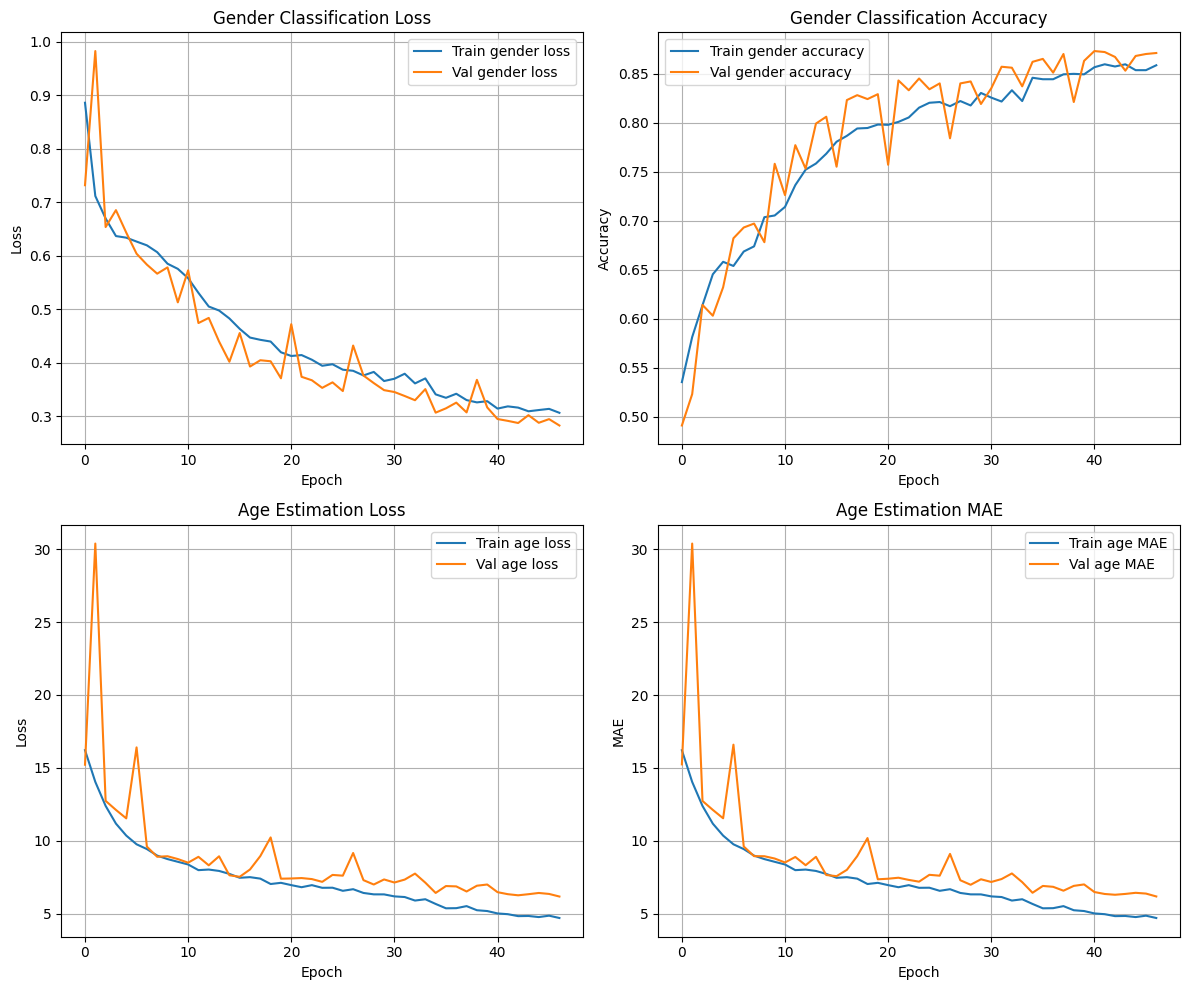
\includegraphics[width=0.80\linewidth]{figure4.png}
    \caption{Learning curves for age and gender tasks. Best Epoch: 47. Training MAE: 4.74, Validation MAE: 6.18. Training gender accuracy: 85.4\%, Validation gender accuracy: 87.1\%}
  \label{figure4}
\end{figure}

\subsection{Learning Curves}
Looking at both learning curves, we notice initial instability in the early epochs, which is a result of a more aggressive learning rate near the beginning. Also, since the CNN is a multi-output problem, it is difficult to simultaneously optimise both age and gender, causing bumps in the graph.

Despite this, looking at the gender learning curve we see that it initially has noise at the start, caused by compromise over the two parameters. Since the age loss has higher weights, the model will move in the direction prioritising minimising the MAE loss, which may cause gender loss to be overlooked. Looking at the validation gender accuracy, we notice that it clearly is converging to a stable value showing no signs of overfitting.

\section{The Pre-trained CNN (Model B)}
\subsection{Model Training and Structure}

\begin{table}[h!]
\centering
\renewcommand{\arraystretch}{1.15}
\begin{tabular}{||l|c|c|c|c||}
 \hline
 Layer & Filters / Units & Output & Kernel Size & Activation fn \\ [0.5ex]
 \hline\hline
 Input image        & -    & $128 \times 128 \times 3$   & -          & -      \\
 \hline\hline
 \multicolumn{5}{||c||}{\textbf{Pre-trained VGG16 feature extractor (frozen)}} \\
 \hline
 Block1 Conv1       & 64   & $128 \times 128 \times 64$  & $3 \times 3$ & ReLU  \\
 Block1 Conv2       & 64   & $128 \times 128 \times 64$  & $3 \times 3$ & ReLU  \\
 Block1 MaxPooling  & -    & $64 \times 64 \times 64$    & $2 \times 2$ & -     \\
 \hline
 Block2 Conv1       & 128  & $64 \times 64 \times 128$   & $3 \times 3$ & ReLU  \\
 Block2 Conv2       & 128  & $64 \times 64 \times 128$   & $3 \times 3$ & ReLU  \\
 Block2 MaxPooling  & -    & $32 \times 32 \times 128$   & $2 \times 2$ & -     \\
 \hline
 Block3 Conv1       & 256  & $32 \times 32 \times 256$   & $3 \times 3$ & ReLU  \\
 Block3 Conv2       & 256  & $32 \times 32 \times 256$   & $3 \times 3$ & ReLU  \\
 Block3 Conv3       & 256  & $32 \times 32 \times 256$   & $3 \times 3$ & ReLU  \\
 Block3 MaxPooling  & -    & $16 \times 16 \times 256$   & $2 \times 2$ & -     \\
 \hline
 Block4 Conv1       & 512  & $16 \times 16 \times 512$   & $3 \times 3$ & ReLU  \\
 Block4 Conv2       & 512  & $16 \times 16 \times 512$   & $3 \times 3$ & ReLU  \\
 Block4 Conv3       & 512  & $16 \times 16 \times 512$   & $3 \times 3$ & ReLU  \\
 Block4 MaxPooling  & -    & $8 \times 8 \times 512$     & $2 \times 2$ & -     \\
 \hline
 Block5 Conv1       & 512  & $8 \times 8 \times 512$     & $3 \times 3$ & ReLU  \\
 Block5 Conv2       & 512  & $8 \times 8 \times 512$     & $3 \times 3$ & ReLU  \\
 Block5 Conv3       & 512  & $8 \times 8 \times 512$     & $3 \times 3$ & ReLU  \\
 Block5 MaxPooling  & -    & $4 \times 4 \times 512$     & $2 \times 2$ & -     \\
 \hline
 GlobalAvgPooling   & -    & $512$                       & -           & -     \\
 Shared FC          & 512  & $512$                       & -           & ReLU  \\
 Shared Dropout     & -    & $512$                       & -           & -     \\
 \hline\hline
 \multicolumn{5}{||c||}{\textbf{Gender Branch}} \\
 \hline
 Gender FC          & 128  & $128$                       & -           & ReLU    \\
 Gender Dropout     & -    & $128$                       & -           & -       \\
 Gender output      & 1    & $1$                         & -           & Sigmoid \\
 \hline\hline
 \multicolumn{5}{||c||}{\textbf{Age Branch}} \\
 \hline
 Age FC             & 256  & $256$                       & -           & ReLU    \\
 Age BatchNorm      & -    & $256$                       & -           & -       \\
 Age Dropout        & -    & $256$                       & -           & -       \\
 Age output         & 1    & $1$                         & -           & Linear  \\
 \hline
\end{tabular}
\caption{Model B architecture: Transfer learning model with VGG16-backbone}
\label{table3}
\end{table}

Model B is a transfer learning model built on top of a pre-trained VGG16 base. This architecture was selected due to its use of a uniform 3x3 convolutional filter that is similar in nature to the custom CNN model. Seeing how a pre-trained model compares with the custom model using a similar architecture helps to make a more direct comparison \cite{rothe2018deep}. The backbone of the model is made up of two sets of double-stacked Conv2D layers, followed by three layers of triple-stacked Conv2D layers, with MaxPooling after each stack. The output of the head of the pre-trained CNN is very similar to that of the custom CNN. Here, we add an additional shared 512-unit fully connected layer so that the model can learn features that benefit both age and gender.

The model is trained in two stages and follows the standard approach of transfer-learning models. The first stage keeps the entire VGG16 backbone frozen and only trains the new heads added for the required outputs. This stage is trained using Adam (learning rate: $5 \times 10^{-4}$), where a larger learning rate and 20 epochs are used since this stage is just used to initialise the weights of the layers added for the custom age and gender output. The losses used are identical to the custom CNN for the same reasons, and similarly for techniques such as He Normal and the activation functions for all stages. The losses for the first learning stage are chosen using a ratio of 0.65 : 0.35, age:gender. This is done so that age starts stronger.

In the second stage, we fine-tune the model, choosing to only freeze the first 7 layers, which correspond to just the double-stacked convolution blocks. This choice was made as a result of experimenting with different values, and the choice of weights in the ratio 0.4:0.6, age:gender, is made to provide a more equal convergence of the two outputs. The learning rate is now lower, using Adam (learning rate: $5 \times 10^{-4}$), and the callbacks are used with longer patience so the fine-tuning stage can explore longer while guarding against overfitting.

\subsection{Learning Curves}

\begin{figure}[ht]
  \centering
  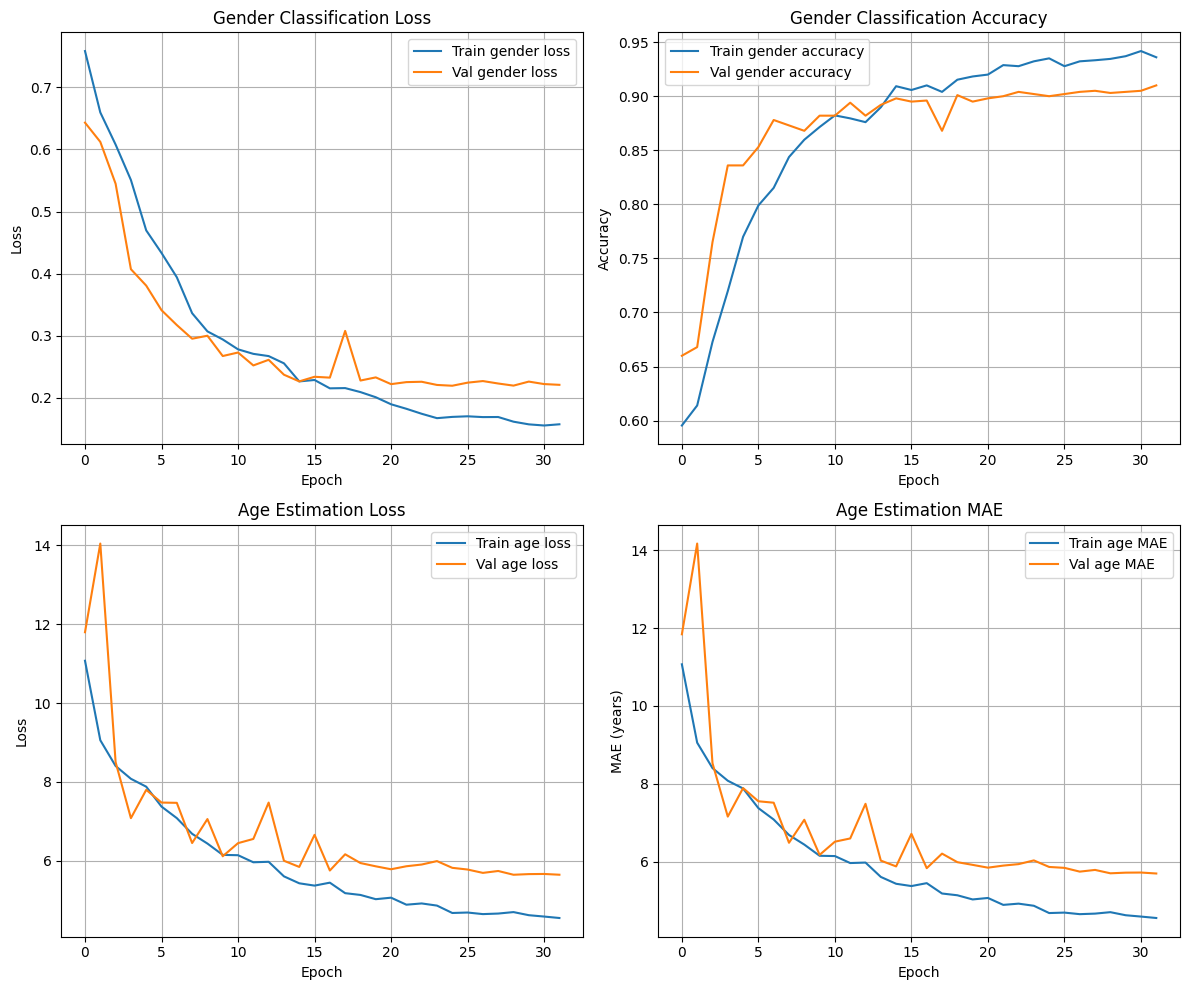
\includegraphics[width=0.80\linewidth]{figure5.png}
    \caption{Learning curves for age and gender tasks. Best Epoch: 34. Training MAE: 4.52, Validation MAE: 5.67. Training gender accuracy: 93.9\%, Validation gender accuracy: 90.7\%}
  \label{figure5}
\end{figure}

Both age and gender learning curves show great improvements compared to the custom CNN. One thing that stands out is that near the beginning it appears that the validation set on the gender learning curve seems to outperform the training data curve. This is mostly down to the pre-trained network having learnt patterns on data that is not augmented and hence the validation data displays better results.

We also see that this network, due to its initial training step, converges at a faster rate, appearing to plateau around the 20–25 epoch mark, despite the low learning rate used. This can be explained by the initial training done on the completely frozen pre-trained network. By allowing the output heads to learn the weights, it greatly sped up the process when it came down to training the model with the unfrozen layers.

Comparing the age and gender learning curves, they appear to converge in a similar timescale, which shows that the weights used to optimise the loss of the model were optimum for both age and gender. Similar appearing curves suggest that there was no overly dominating feature in this example. This could be attributed to the joint dense layer allowing the model to learn features which are optimum for both the gender and age.

\section{Summary and discussion} 
Both models were relatively effective in the task of gender classification however determining the age is yet to be achieved accurately enough. The pre-trained model was able to outperform the custom CNN in both metrics as expected however the fact that the learning curves showed plateauing and converging signs meant it was more a problem with the data than the network itself. \autoref{figure1} and \autoref{table1} both display the data we are given and we can understand that there is clear bias towards ages (20-29) and a slight bias towards males. The fact that the younger generating is over represented means that the CNN will also reflect that bias towards the age and gender group presenting problems. 
\newpage{}
\bibliographystyle{ieeetr}
\bibliography{references}

\end{document}